\section{Introduction}
\begin{frame}{Introduction}
\framesubtitle{Text Classification}
\begin{itemize}
\item Text Classification is the process of categorizing text documents into predefined classes based on their content
\item Its applications: document organization, news filtering, spam detection, opinion mining, and computational phenotyping
\end{itemize}

\begin{figure}
\centering
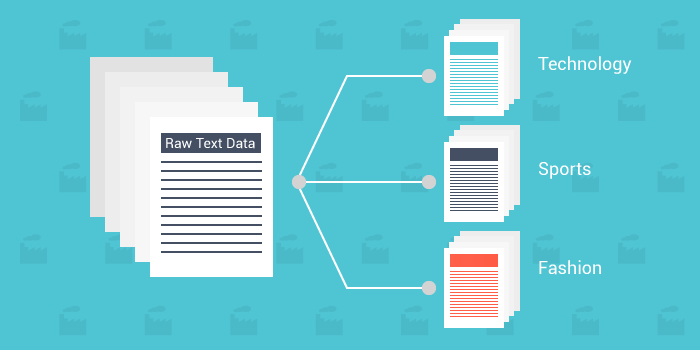
\includegraphics[width=80mm,scale=0.7]{img/TC_example.png}
\caption{Example of Text Classification}
\label{fig:example}
\end{figure}
\end{frame}

\begin{frame}{Introduction}
\framesubtitle{Observation and Motivation}
Observation:
\begin{itemize}
\item The depth necessitates a large number of parameters that must be loaded into memory, limiting to the training phase and may pose challenges in real-world scenarios (inference under low-latency constraints or fine-tuning with limited resources.)
\end{itemize}

Motivation: 
\begin{itemize}
\item Creating more compact models with fewer parameters (such as knowledge distillation based models)
\end{itemize}
\end{frame}

\begin{frame}{Introduction}
\framesubtitle{Contribution}
\begin{itemize}
\item Our proposal can be more appropriate for real-world appliances by its viability of inferencing under low-latency constraints or well-functioning in limited computational resources.
\item Our experimental results demonstrate that the proposal achieves comparable performance to SOTA text classification methods on several benchmark datasets.
\end{itemize}
    
\end{frame}